%% Bioinformatics mixer blitz using beamer and biblatex (bibtex backend)
%% AG Schissler, 28 Jan 2017
%% Last modified 6 Feb 2018

%%%% Preamble
%% Beamer specifications
%\documentclass[aspectratio=169]{beamer}
\documentclass{beamer}
\usepackage{beamerthemeshadow}
\setbeamertemplate{navigation symbols}{} %remove navigation symbols

%% make larger beamer buttons
%% http://tex.stackexchange.com/questions/108174/beamergotobutton-size
\usepackage{tikz}
\setbeamertemplate{button}{\tikz
  \node[
  inner xsep=10pt,
  draw=structure!80,
  fill=structure!50,
  rounded corners=4pt]  {\Large\insertbuttontext};}

%% title fields
\title[Correlated paired-sample gene set analysis]{Gene set analysis of correlated, \\paired-sample transcriptome data \\to enable precision medicine}  
\author{A.~Grant~Schissler, PhD}
% \date{16 Feb 2017}
%\date{}

\institute[]
{
  \footnotesize{Department of Mathematics \& Statistics\\
  University of Nevada, Reno}
}
% Includes for frame package
\usepackage{framed,color}
\definecolor{shadecolor}{rgb}{0.5,0.5,0.5}

% Make a custom block
\newenvironment<>{customBlock}[1]{%
  \begin{actionenv}#2%
      \def\insertblocktitle{#1}%
      \par%
      \mode<presentation>{%
        \setbeamercolor{block title}{fg=white,bg=orange!20!black}
       \setbeamercolor{block body}{fg=black,bg=olive!50}
       \setbeamercolor{itemize item}{fg=orange!20!black}
       \setbeamertemplate{itemize item}[triangle]
     }%
      \usebeamertemplate{block begin}}
    {\par\usebeamertemplate{block end}\end{actionenv}}

  \usepackage[framemethod=tikz]{mdframed}

  \newmdenv[tikzsetting={draw=black,fill=white,fill opacity=0.7, line width=4pt},backgroundcolor=none,leftmargin=0,rightmargin=0,innertopmargin=4pt,skipbelow=\baselineskip,%
skipabove=\baselineskip]{TitleBox}
%http://tex.stackexchange.com/questions/38281/transparent-background-for-mdframed-environment


%%\pgfdeclareimage[width=\paperwidth]{mybackground}{figures/NxT_MD_fig1_title.pdf}
%%
%%\setbeamertemplate{title page}{
%%
%%        \begin{picture}(0,0)
%%
%%            \put(-30,-163){%
%%                \pgfuseimage{mybackground}
%%            }
%%
%%            \put(0,-110.7){%
%%                \begin{minipage}[b][45mm][t]{226mm}
%%                    \usebeamerfont{title}{\inserttitle\par}
%%                \end{minipage}
%%            }
%%            \end{picture}
%%
%%    }
%%

%%%%%% Reference management (such a pain)
%% biblatex for references
%http://tex.stackexchange.com/questions/128810/bibliography-with-only-initials-of-names
\usepackage[backend=biber, style=authoryear,
autocite=footnote, firstinits=true, maxcitenames=2, mincitenames=2]{biblatex}
\addbibresource{blitz_lib.bib}
%\newcommand*{\footlessfullcite}{\AtNextCite{\renewbibmacro{title}{}\renewbibmacro{in:}{}}\footfullcite}
%\addtobeamertemplate{footnote}{\vspace{-6pt}\advance\hsize-0.5cm}{\vspace{6pt}}

%% http://tex.stackexchange.com/questions/194078/add-journal-name-to-biblatex-references
\renewbibmacro*{cite}{%
  \iffieldundef{shorthand}
    {\ifthenelse{\ifnameundef{labelname}\OR\iffieldundef{labelyear}}
       {\usebibmacro{cite:label}%
        \setunit{\addspace}}
       {\printnames[last-first]{labelname}%
        \setunit{\nameyeardelim}}%
     \usebibmacro{cite:labelyear+extrayear}%
     \setunit{\addcomma\space}%
     \usebibmacro{journal}}
   {\usebibmacro{cite:shorthand}}}

%% suppress pages in cites
%% http://tex.stackexchange.com/questions/113039/trying-to-suppress-urls-with-biblatex-using-a-simple-persons-method
%\AtEveryCitekey{\clearfield{pages}}
%\AtEveryCitekey{\clearfield{title}}

%%%% use short journal name
\DeclareSourcemap{
  \maps[datatype=bibtex]{
    \map[overwrite]{ % Notice the overwrite: replace one field with another
      \step[fieldsource=shortjournal,fieldtarget=journaltitle]
    }
  }  
}
 
%%%% make footnotes
%%%% http://tex.stackexchange.com/questions/44217/how-can-i-stop-footcite-from-hijacking-my-beamer-columns
%\addtobeamertemplate{footnote}{\vspace{-6pt}\advance\hsize-0.5cm}{\vspace{6pt}}
%\makeatletter
% Alternative A: footnote rule
%%\renewcommand*{\footnoterule}{\kern -3pt \hrule \@width 2in \kern 8.6pt}
%\makeatother
%%

%% Other packages for typesetting
\usepackage{array}
\usepackage[none]{hyphenat}

%% cute symbols
\usepackage{marvosym}

%% A few new commands
\newcommand*{\barbar}[1]{\overline{\overline{#1}}}
%%%%%%%%%%%% smaller \overline (NB asymmetric emph. to right)
\newcommand{\overbar}[1]{\mkern 3mu\overline{\mkern-3mu#1\mkern-1.mu}\mkern 1.mu}

%----------------------------------------------------------------------------------------
\begin{document}

{  \usebackgroundtemplate{\includegraphics[width=1.0\paperwidth]{figures/NxT_MD_fig1_title.pdf}}
  \begin{frame}[plain] 

     \vskip60pt
  \begin{TitleBox}
    {\huge \inserttitle} 
    \vskip5pt
    {\large\insertauthor}\\
    \insertinstitute\\
    %{\footnotesize \href{http://twitter.com/adaptive_plant}{{\FA \faTwitter} adaptive\_plant}
    %\href{http://www.falsters.net/daniel}{{\FA \faHome} www.falsters.net/daniel}
    %\href{mailto: daniel.falster@mq.edu.au}{{\FA \faEnvelope}  daniel.falster@mq.edu.au}
    % }
    \vskip3pt
%%    {\footnotesize Statistical advisor:~Dr.~Walter W.~Piegorsch}\\
%%        {\footnotesize Biomedical informatics advisor:~Dr.~Yves A.~Lussier}
    {\footnotesize
      \Email\href{mailto: aschissler@unr.edu}{aschissler@unr.edu}\\
      \Mundus\href{http://www.grantschissler.com}{www.grantschissler.com}
    }
   \end{TitleBox}

 \end{frame}
 \note{Welcome all to my doctoral defense! Today, my job is to both share my research over the past 3 years and to justify the ideas and methods.}
 \note{As the title suggests, my research focused on a pretty narrow statistical topic but with promising applications in precision medicine.}
 \note{The title could make anywhere from perfect sense to non-sense for each of you, but I hope everyone can take away the main ideas.}
}

%% the title page
%% \begin{frame}[plain]
%% \titlepage
%% \end{frame}

%% Outline
%%\begin{frame}
%%  \frametitle{Presentation outline}
%%    \tableofcontents
%%  % \tableofcontents[pausesections]
%%  \note{As there is a lot to cover, let me step through an outline of this talk.}
%%  \note{First, quickly provide some motivating data and essential background.}
%%  \note{Then, we\rq ll discuss in detail the statistical method development and evaluation.}
%%  \note{Time allowing, present some key results, visualizations, and an R implementation.}
%%  \note{Lastly, I\rq ll quickly summarize the work and future directions.}
%%\end{frame} 
%%

%%%% Part I: Precision medicine motivation
\section{Motivating data \& background}
\subsection{Motivating data}
\begin{frame}\frametitle{Example paired RNA-seq\addtocounter{footnote}{-2}\footnotemark ~quantified mRNA (normalized) expression data in a gene set\footnotemark}
  \begin{table}
\label{tab:TNBCdata}
\begin{tabular}{l|ccc}
\hline
Gene & Case expression & Baseline expression & Difference\\
\hline
  \emph{CYP4A11}   & 0.00  & 3.71  & -3.71 \\
  \emph{AGTR1}     & 6.13  & 7.86  & -1.73 \\
  \emph{OR51E2}    & 2.90  & 1.54  & 1.36 \\
  \emph{CYP11B2}   & 0.00  & 0.00  & \phantom{-}0.00 \\
  \emph{PTPRO}     & 3.72  & 6.22  & -2.50 \\
  \emph{CYP4F2}    & 0.00  & 0.40  & -0.40 \\
  \emph{AGT}       & 8.40  & 7.89  & \phantom{-}0.52 \\
  \emph{$\ldots$}       & $\ldots$  & $\ldots$  & $\ldots$ \\
  \emph{SERPINF2}  & 6.38  & 9.57  & -3.19 \\
\hline
\end{tabular}
\end{table}
\addtocounter{footnote}{1}\footcitetext{Wang2009}
\addtocounter{footnote}{1}\footcitetext{Ashburner2000}
\note{The data of interest can be simply represented in a table. Imagine there are two biological samples:~A case sample and a baseline sample <point to first two columns>.}
\note{From these samples, messenger RNA expression are quantified for genomic locations, which for the sake of brevity, Ill call genes <point to rows>.}
\note{These genes are not selected randomly, they are grouped together based on functional annotations housed in a knowledgebase. Here these genes help to regulate blood pressure.}
\note{Ill say more precisely the research questions of interest, but informally we want to understand the amount and variation of differentially expression <point to third column>.}
\note{The major issues are that n \<< p, baseline and case are often sampled from the same organism, and gene are co-expressed (correlated).}
%% transition to joke
\note{Im not sure what you think about these data, but a can tell you as a junior grad student how I felt...}
\end{frame}

\begin{frame}\frametitle{A statistician\rq s nightmare}
  \begin{figure}[htb]
  \centering
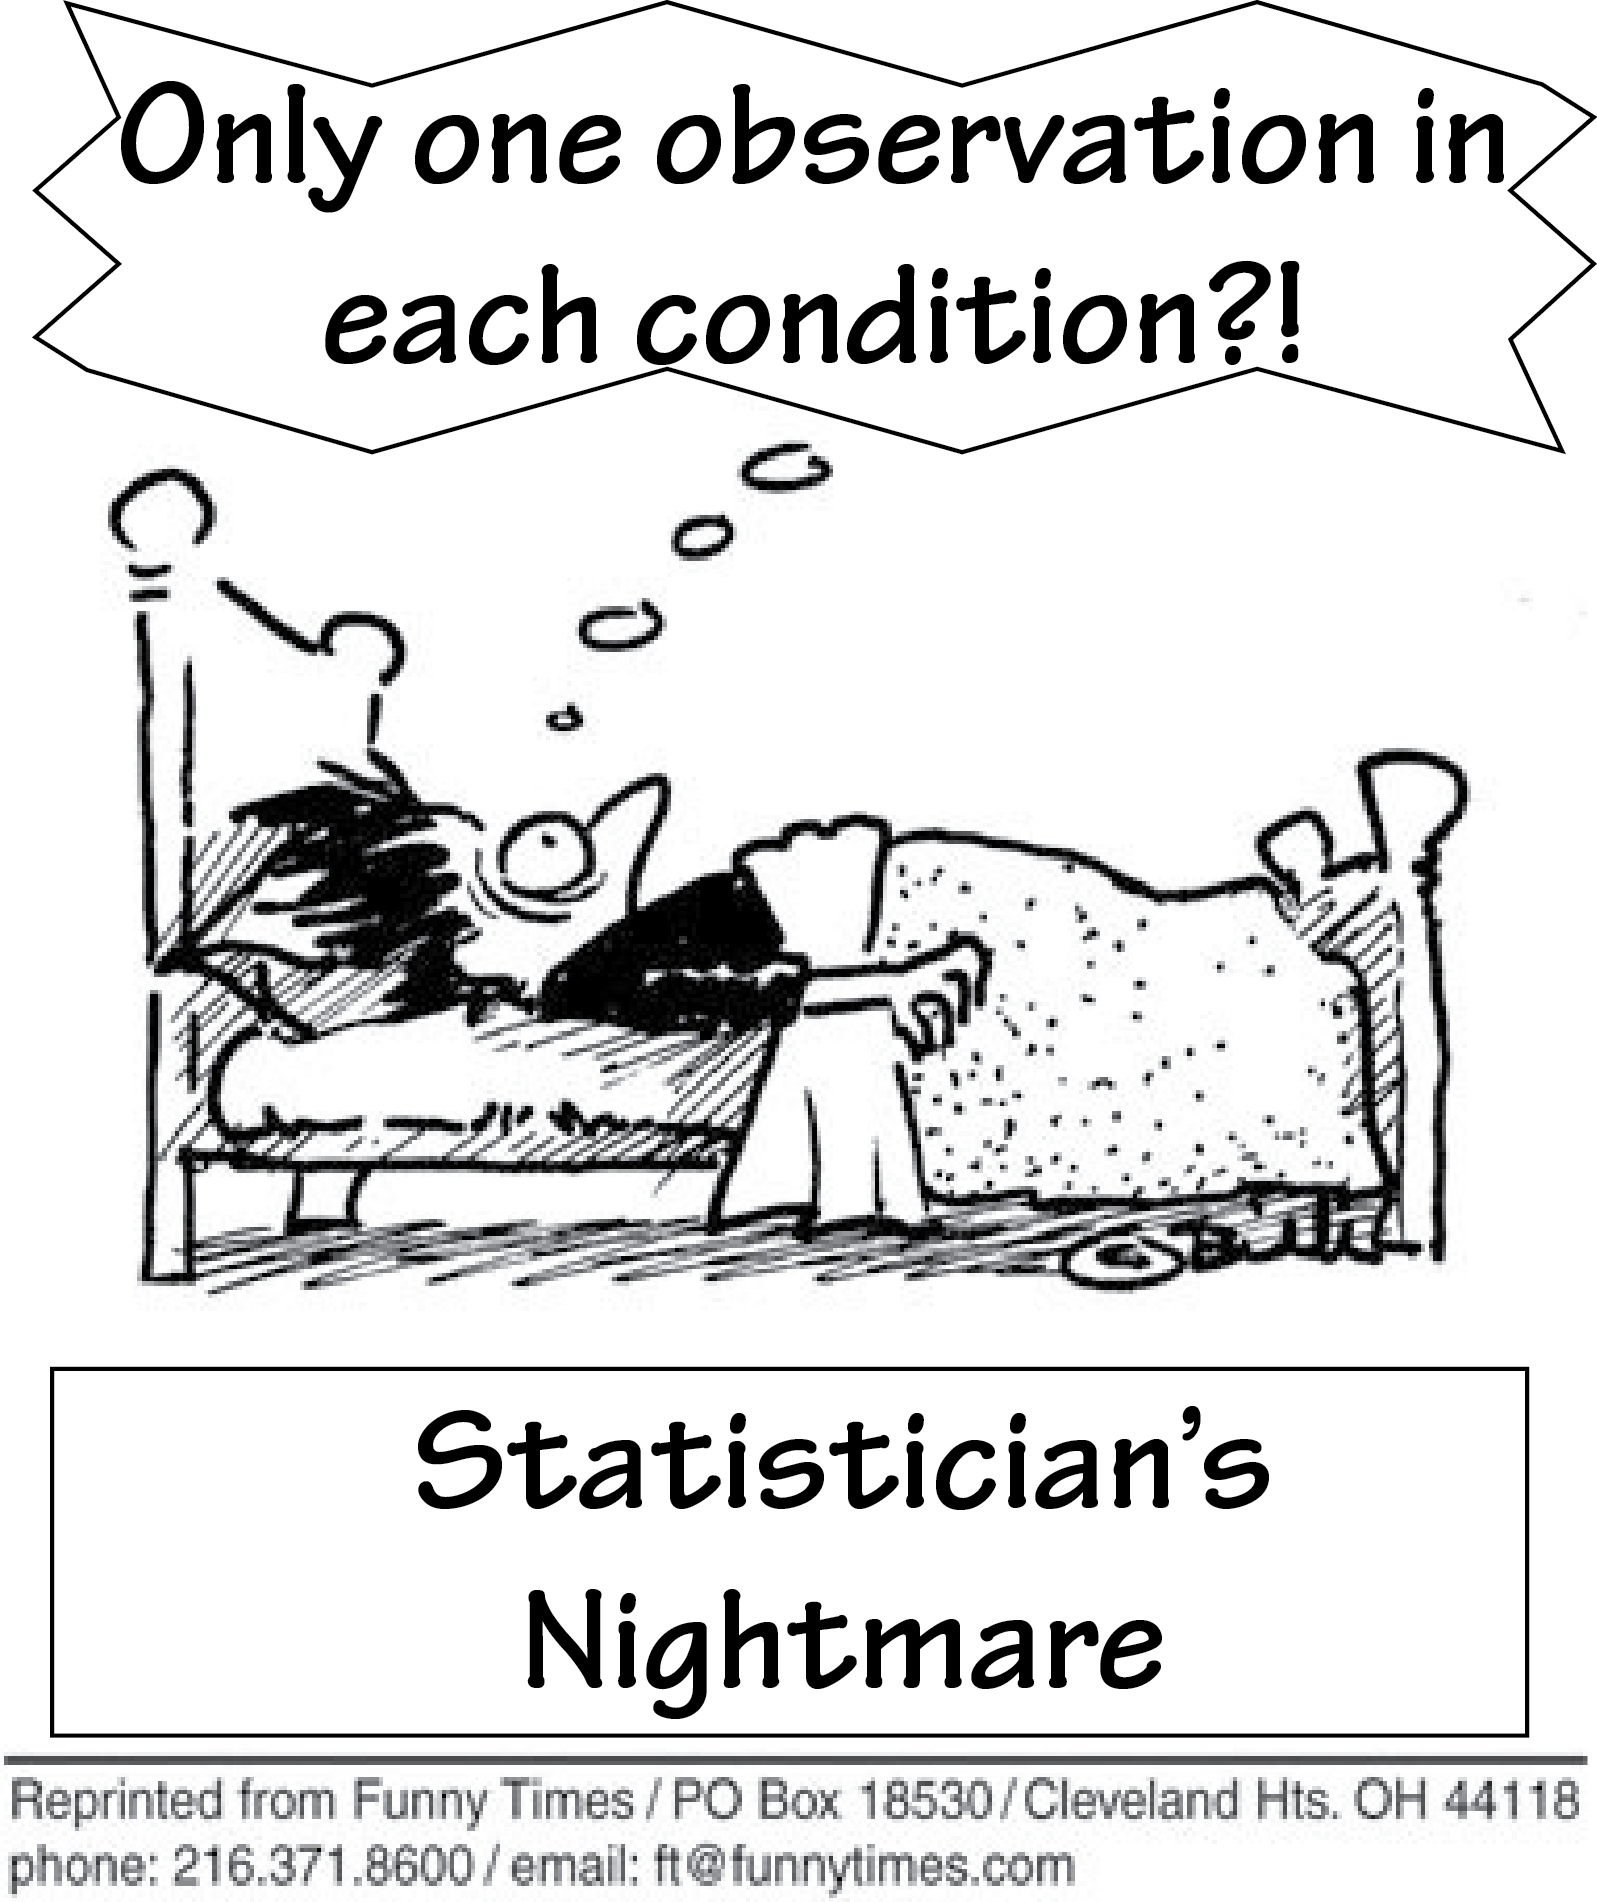
\includegraphics[keepaspectratio,width=\textwidth,height=0.8\textheight]{figures/nightmare_cartoon_v2.png}
   \end{figure}
   \note{Practice issues: correlated, within-patient}
   \note{Philosophical: what's my population, what am I inferring}
\end{frame}

%%\begin{frame}\frametitle{Why is studying individualized dysregulation important?}
%%  \begin{itemize}
%%  \item Cohort-derived cancer biomarkers are notoriously difficult to produce effective therapies for all patients\footcite{Kern2012}.
%%  \item This leads to the recent attention on developing precision medicine\footcite{Hamburg2010}.
%%  \item Some even speculate that N-of-1 is the ``ultimate strategy for individualizing medicine''\footcite{Lillie2011}.
%%  \item Moreover, small studies are cost efficient and allow investigation into rare disease.
%%  \end{itemize}
%%\end{frame}

\subsection{Interdisciplinary work products}
\begin{frame}\frametitle{Interdisciplinary focus:~Biomedical questions of interest and work products}
  \begin{itemize}
    %\pause
  %\item How differentially expressed are the genes and corresponding gene sets between the pair of samples?
   % \begin{itemize}
    \item {Can you provide a meaningful effect size\footnotemark?}
    %\end{itemize}
     %   \pause
  %\item {How can I interpret uncertainty in these measurements?}
    %\begin{itemize}
    \item {Can you provide a measure of uncertainty (e.g., P-value\footnotemark?)}
    %\end{itemize}
        \pause
  \item {How can these statistics be used in research and practice?}
    \begin{itemize}
      \addtocounter{footnote}{-2}
      %\pause
    \item {\alert{Single-subject inferences}:~breast cancer patients\footnotemark$^{,}$\footnotemark, HIV\footnotemark.}
      \addtocounter{footnote}{0}
      %\pause
    \item {single-cell data\footnotemark.}
      \addtocounter{footnote}{0}
    %\item {Novel visualizations for paired differential expression\footnotemark.}
      \item {R package\footnotemark}.
    \end{itemize}
  \end{itemize}

\vskip-5pt \addtocounter{footnote}{-5}\stepcounter{footnote}\only<1->{\footcitetext{Schissler2015}}
  \addtocounter{footnote}{0}\stepcounter{footnote}\only<1->{\footcitetext{Schissler2017}}
  \addtocounter{footnote}{0}\stepcounter{footnote}\only<2->{\footcitetext{Li2016}}
  \addtocounter{footnote}{0}\stepcounter{footnote}\only<2->{\footcitetext{Schissler2016}}
\addtocounter{footnote}{0}\stepcounter{footnote}\only<2->{\footnotetext{http://www.lussiergroup.org/publications/N-of-1-pathways}}
  \note{Our stats program focusing on interdisciplinary collaboration and so I tried to address to provide statistically reasonable solutions to key questions.}
  \note{These work products proceeded in a non-linear fashion, but at the end of the day this how I would summarize the work.}
  \note{How much differential expression?}
  \note{How deal with uncertainty?}
  \note{How to translate the ideas to context domains?}
  \note{paraphrase the points.}
\end{frame}

%%\subsection{Gene set analysis}
%%\begin{frame}\frametitle{Gene set analysis in biomedical research}
%%    \vskip-10pt
%%  \begin{itemize}
%%  \item Gene set analyses\footcite{Huang2009} give mechanistic interpretation by aggregating gene-level results.
%%  \item {Widely-used methods:~GSEA\footcite{Subramanian2005} and DEG + enrichment\footcite{Beibarth2004}}
%%  \end{itemize}
%%  \vskip-6pt
%%  \pause
%%    \begin{block}{Example ontology:~Gene Ontology Biological Processes (GO-BP)}
%%    \begin{center}
%%      \begin{tabular}{lll}
%%        GO-ID & Description & Gene\\
%%        \hline
%%        GO:0000002 & mitochondrial genome maintenance & TP53\\
%%        GO:0000002 & mitochondrial genome maintenance & OPA1\\
%%        \vdots & \vdots & \vdots\\
%%        GO:2001317 & kojic acid biosynthetic process & NPPA\\
%%      \end{tabular}
%%    \end{center}
%%  \end{block}
%% \note{Some brief background on gene set analysis. Gene set analysis is ubiquitous}
%%\end{frame}
%%

%%\subsection{The N-of-1-{\itshape pathways} framework}
%%\begin{frame}\frametitle{The N-of-1-{\itshape pathways} framework\addtocounter{footnote}{-1}\footnotemark}
%%  \begin{figure}[htb]
%%    \centering
%%\includegraphics[keepaspectratio,width=\textwidth,height=0.6\textheight]{figures/N-of-1-pathways-dep-flowchart.pdf}
%%\end{figure}
%%\pause
%%The first attempt at a testing procedure employed a Wilcoxon signed-rank test\footcite{Gardeux2014}.
%%\note{Smart dimension reduction of the transcriptome}
%%\note{Move quickly on this slide.}
%%\note{Mention the shortcomings}
%%\end{frame}
%%
%%%% Part II: Correlation-adjusted analytics
\section{Correlation-adjusted analytics}

\subsection{Only time for one picture...}
\begin{frame}\frametitle{Illustrative representation of methods}
      \begin{figure}[htb]
  \centering
\includegraphics[keepaspectratio,width=\textwidth,height=0.8\textheight]{figures/NxT_MD_fig1_summary.pdf}
   \end{figure}
\end{frame}
%%
%%\frame{\tableofcontents[currentsection]}
%%\subsection{Effect size:~average Mahalanobis distance (MD)}
%%
%%\begin{frame}\frametitle{Key picture:~distance from null-response line}
%%       \begin{columns}[c]
%%   \begin{column}{6cm}
%%    \begin{figure}[htb]
%%    \centering
%%\includegraphics[keepaspectratio,width=0.8\columnwidth]{figures/NxT_MD_fig1.pdf}
%%\end{figure}
%%   \end{column}
%%   \begin{column}{6cm}
%%     \pause
%%     Some notation:\\
%%          \vspace{0.3cm}
%%     $\Delta X_{i} = (B_{i}, C_{i}) - (B_{i}, B_{i}) = (0, C_{i} - B_{i})$\\
%%     \vspace{0.3cm}
%%     $\hat{\Sigma} = \left( \begin{matrix}
%%         S_{B}^{2} &  S_{BC}\\
%%         S_{CB} &  S_{C}^{2}\\
%%       \end{matrix} \right)$\\
%%          \vspace{0.3cm}
%%     $\tau=\frac{1}{S_{B}^{2}S_{C}^{2}-(S_{BC})^{2}}$.
%%   \end{column}
%%   \end{columns}
%%\end{frame}
%%
%%\begin{frame}\frametitle{Calculating the signed Mahalanobis distance}
%%  By definition, the squared, vertical Mahalanobis distance for gene $i$ is the quadratic form
%%     \begin{eqnarray*}
%%       \delta_{i}^{2} = & (\Delta X_{i})^{T}\hat{\Sigma}^{-1}\Delta X_{i}& \\
%%        = & \tau \left( \begin{matrix} 0 & C_{i} - B_{i} \end{matrix}\right) \left( \begin{matrix}
%%         S_{C}^{2} &  -S_{BC}\\
%%         -S_{CB} &  S_{B}^{2}\\
%%       \end{matrix} \right)  \left( \begin{matrix}
%%         0\\
%%         C_{i}- B_{i}\\
%%       \end{matrix} \right) & \\
%%       = & \tau (C_{i} - B_{i})^{2} S_{B}^{2} & (S_{BC} = S_{CB}) \\
%%       = & \frac{S^{2}_{B}}{S^{2}_{B}S^{2}_{C}-(S_{BC})^{2}}(C_{i} - B_{i})^{2} & \\
%%     \end{eqnarray*}
%%     \pause
%%       \centering \hskip-30pt Then, the observed signed Mahalanobis distance is\\
%%\hskip-30pt $\delta_{i} = \sqrt \frac{S^{2}_{B}}{S^{2}_{B}S^{2}_{C}-(S_{BC})^{2}}(C_{i} - B_{i})$
%%\end{frame}
%%
%%\begin{frame}\frametitle{Motivation and interpreting the MD score}
%%         \begin{columns}[c]
%%   \begin{column}{5cm}
%%\begin{eqnarray*}
%%  \delta_{i} = & \sqrt{\frac{S^{2}_{B}}{S^{2}_{B}S^{2}_{C}-(S_{BC})^{2}}}(C_{i} - B_{i}) & \\
%%  = & \sqrt{\frac{S^{2}_{B}}{S^{2}_{B}S^{2}_{C}-(S_{B}S_{C}r_{BC})^{2}}}(C_{i} - B_{i}) & \\
%%= & \sqrt{\frac{1}{S^{2}_{C}(1-r^{2}_{BC})}}(C_{i} - B_{i}) & \\
%%\end{eqnarray*}
%%%\pause
%%% Refer to the sample mean $\bar{d} = G^{-1}\sum_{i=1}^{G}d_{i}$\\ as the ``MD score''\footnotemark.
%%\end{column}
%%\begin{column}{6.5cm}
%%  \pause
%%\begin{itemize}
%%\item Small changes in a tightly regulated pathway are more impactful.
%%  \pause
%%\item Down-weights more variable pathways in the case sample.
%%  \pause
%%\item A pathway-level \alert{effect size} of variance-covariance-adjusted differential expression is the sample mean, $\bar{\delta} = \sum_{i=1}^{G}\delta_{i}/G$.\\ \pause(referred to as the ``MD score''\footnotemark).\\
%%  % \item and between-sample covariance-adjusted average log$_{2}$ fold-change of mRNA expression.
%%  %\item The MD score can be interpreted as the between-sample, covariance-adjusted average log$_{2}$ fold-change of mRNA expression.
%%  \end{itemize}
%%\end{column}
%%\end{columns}
%%\only<5->\footcitetext{Schissler2015}
%%\end{frame}
%%
%%\subsection{Hypothesis testing:~the clustered-{\itshape T} statistic}
%%
%%\begin{frame}\frametitle{Standard error estimation/Gene set testing}
%%  \begin{columns}[T]
%%    \begin{column}{0.5\columnwidth}\small
%%%%      \pause
%%          $H_{0}$:~Pathway is not differentially expressed. \\
%%          $H_{a}$:~Pathway is differentially expressed.\\
%%          \pause
%%          \begin{itemize}
%%          \item {But mRNAs are likely co-expressed (correlated) within pathways.}
%%                        \pause
%%          \item{Accounting for inter-gene correlation in gene set testing is an active area of research\footnotemark$^{,}$\footnotemark.}
%%
%%          \end{itemize}
%%
%%  \note{Now I wish to quantify the evidence that the MD score is different from 0, indicating differential pathway expression.}
%%  \note{ Note the mRNAs (genes) are the observations in this framework.}
%%  \note{ But mRNAs are co-expressed (correlated).}
%%  \note{ Assuming independence could lead to very poor estimation of standard error of the sample mean (or the MD score which is simply a scaled sample mean).}
%%  \note{Derive a correlation-adjusted reference sampling distribution for the MD score.}
%%  \note{But with $N=1$ (a single vector of gene-wise differences) makes estimating the variance-covariance matrix difficult.}
%%
%%\end{column}
%%\begin{column}{0.45\columnwidth}
%%  \pause
%%      \begin{figure}
%%      \centering
%%\includegraphics[keepaspectratio,width=0.9\columnwidth]{figures/cT_r_hist_fig_S1_small.pdf}
%%      \end{figure}
%%    \end{column}
%%  \end{columns}
%%  \addtocounter{footnote}{-2}
%% \stepcounter{footnote}\only<3->\footcitetext{Wu2012}
%% \stepcounter{footnote}\only<3->\footcitetext{Tamayo2016}
%%\end{frame}
%%
%%\begin{frame}\frametitle{Major issue:~inter-gene correlations complicate testing}
%%  \centering So how to proceed???
%%\end{frame}
%%
%%
%%%%\begin{frame}\frametitle{A tool:~a cluster-correlated variance estimator}
%%%%      
%%%%      \begin{block}{General notation \& assumptions}
%%%%        \begin{itemize}
%%%%        \item{Let $d_{jk}$ be the $k^{\text{th}}$ observation ($k = 1,2,\ldots,n_j$) in the $j^{\text{th}}$ cluster ($j = 1,2,\ldots,m$).}
%%%%          \item{And let $d_{j}=\sum_{k}d_{jk}$ and $\bar{d}=\sum_{m}d_{j}/m$.}
%%%%        \item{Assume that $E[d_{jk}]=0$.}
%%%%        \item{And that $cov[d_{jk},d_{jk^{\prime}}]=\sigma_{jkk^{\prime}}$,~$cov[d_{jk},d_{j^{\prime}k^{\prime}}]=0$ when $j\neq j^{\prime}$.}
%%%%        \end{itemize}
%%%%      \end{block}
%%%%
%%%%      \begin{block}{An unbiased variance estimator for a linear statistic\footnotemark}
%%%%        \begin{equation*}
%%%%\label{eq:var}
%%%%\widehat{\text{Var}}\left[\sum_{j}\sum_{k}d_{jk}\right] = \frac{m}{m-1}\sum_{j=1}^m(d_j - \bar{d})^2
%%%%\end{equation*}
%%%%\end{block}
%%%%\footcitetext{Williams2000}
%%%%
%%%% talking points
%%%%\note{between-cluster variance}
%%%%  \note{I explored much theory and tools to account for correlated observations.}
%%%%  \note{But with $N=1$ (a single vector of gene-wise differences) makes estimating the variance-covariance matrix difficult.}
%%%%  \note{Eventually, I stumbled across a robust variance estimator for the grand sum (which can be scaled to a mean) when given cluster-correlated data\footcite{Williams2000}.}
%%%%  \note{The beauty of the estimator lies in the very general assumptions - the variance can be heteroscedastic, both within and between clusters. Moreover, dependence (covariance) among observations within clusters is arbitrary.}
%%%%    \note {Even better, variances or covariances need \textbf{not} be estimated.}
%%%%\end{frame}
%%
%%
%%%%\begin{frame}\frametitle{A strategy for developing a hypothesis test}
%%%%  \begin{itemize}
%%%%  \item{Derive a correlation-adjusted reference sampling distribution for the MD score.}
%%%%
%%%%  \item{But with $N=1$ (a single vector of gene-wise differences) makes estimating the variance-covariance matrix difficult.}
%%%%  \end{itemize}
%%%%  
%%%%\end{frame}
%%
%%
%%\begin{frame}\frametitle{Notation to develop the clustered-{\itshape T} statistic}
%%    \begin{tabular}{r | c | l }
%%      Concept & Symbol & Definition \\
%%      \hline \hline
%%      Gene-wise difference & $D_{jk}$ & $C_{jk} - B_{jk}$ \\
%%      Cluster index & $j$ & $j = 1,2,\ldots,m$ \\
%%      Observation index & $k$ & $k = 1,2,\ldots,n_j$ \\
%%      Total number of genes & $G$ & $G = \sum_{j} n_{j}$ \\
%%      Grand sum & $D_{\scriptscriptstyle{++}}$ & $\sum_j \sum_k D_{jk}$ \\
%%      Grand mean & $\barbar{D}$ & $D_{\scriptscriptstyle{++}}/G$ \\
%%      Cluster sum & $D_{j\scriptscriptstyle{+}}$ & $\sum_k D_{jk}$ \\
%%      Cluster mean & $\overbar{D}$ & $\sum_j D_{j\scriptscriptstyle{+}}/m$ \\
%%      Sample variance & $S_{D}^{2}$ & $\frac{1}{m-1}\sum_j(D_{j\scriptscriptstyle{+}} - \overbar{D})^2$\\
%%\end{tabular}
%%\end{frame}
%%
%%%% 
%%%%
%%%%\begin{frame}\frametitle{The clustered-{\itshape T} statistic}
%%%%Let $D_{jk} = C_{jk} - B_{jk} $ be the $k^{\text{th}}$ gene-wise case-to-baseline difference ($k = 1,2,\ldots,n_j$) in the $j^{\text{th}}$ cluster ($j = 1,2,\ldots,m$) from a total of $G = \sum_{j} n_{j}$ genes in the target pathway.  Also let $D_{\scriptscriptstyle{++}} = \sum_j \sum_k D_{jk}$ be the grand sum, $D_{j\scriptscriptstyle{+}} = \sum_k D_{jk}$ be the $j^{\text{th}}$ cluster sum, $\overbar{D} = \sum_j D_{j\scriptscriptstyle{+}}/m$ be the mean difference across clusters, and $\barbar{D} = D_{\scriptscriptstyle{++}}/G$ be the grand mean. Lastly, take $S_D^{2}$ as the sample variance $\frac{1}{m-1}\sum_j(D_{j\scriptscriptstyle{+}} - \overbar{D})^2$ across clusters.  (If desired, these expressions translate in a straightforward fashion when pre-determined, cluster-specific weights, $w_j$, are available to differentially weight the clusters; e.g., use $\overbar{D}_w = \sum_j w_j D_{j\scriptscriptstyle{+}}/ \sum_j w_j$, etc.)
%%%%\end{frame}
%%%%
%%
%%\begin{frame}\frametitle{The clustered-{\itshape T} statistic; robust variance estimator}
%%      \begin{block}{Assume centered, cluster-correlated data}
%%        \begin{itemize}
%%        \item{$E[D_{jk}]=0$}.
%%        \item{$cov[D_{jk},D_{jk^{\prime}}]=\sigma_{jkk^{\prime}}$}.
%%        \item{$cov[D_{jk},D_{j^{\prime}k^{\prime}}]=0$ when $j\neq j^{\prime}$}.
%%        \end{itemize}
%%      \end{block}
%%\pause
%%      \begin{block}{Then an unbiased variance estimator\footnotemark~for the grand sum is}
%%        \begin{equation*}
%%\label{eq:var}
%%\widehat{\text{Var}}[D_{\scriptscriptstyle{++}}] = \frac{m}{m-1}\sum_{j=1}^m(D_{j+} - \overbar{D})^2.
%%\end{equation*}
%%\end{block}
%%\pause
%%\centering Clearly, $\widehat{\text{Var}}[D_{\scriptscriptstyle{++}}] = mS_D^2$.
%%\footcitetext{Williams2000}
%%\end{frame}
%%
%%
%%\begin{frame}\frametitle{The clustered-{\itshape T} statistic: hypotheses}
%%  Denote $\mu = E\left(\barbar{D}\right)$ and let this quantity represent the true magnitude of pathway differential expression.\\
%%  \vskip6pt
%%  \begin{block}{Then the statistical hypotheses of interest are}
%%    \begin{equation*}
%%      \label{eq:hypotheses}
%%      \begin{array}{rl}
%%        H_{0}: & \mu = 0 \\
%%        H_{a}: & \mu \neq 0 \ .
%%      \end{array}
%%    \end{equation*}
%%  \end{block}
%%\end{frame}
%%
%%\begin{frame}\frametitle{The clustered-{\itshape T} statistic: reference distribution}
%%  
%%      \begin{block}{Modeling assumptions under $H_0$}
%%        \begin{itemize}
%%        \item{Conditional on the cluster assignments.}
%%        \item{Further assume $D_{j\scriptscriptstyle{+}} \sim N(0, \sigma^2)$.}
%%        \end{itemize}
%%      \end{block}
%%\pause
%%      \begin{block}{Then the clustered-$T$ statistic\only<3->{\footnotemark}}
%%\begin{equation*}
%%  \label{eq:tstat}
%%T =  \frac{\overbar{D}}{S_D/\sqrt{m}}
%%\end{equation*}
%%follows $T \sim t(m-1)$ under $H_0$. \\
%%A (two-sided) P-value is $2\times\text{Pr}[t(m-1) \ge |T|]$.
%%\end{block}
%%\pause
%%\only<3->{\footnotetext{Inferences using $T$ apply to $\barbar{D}$ and the MD score as both are constant scalings of $\overbar{D}$.}}
%%\end{frame}
%%
%%\subsection{Simulating pathways to evaluate operating characteristics}
%%
%%\begin{frame}\frametitle{Simulating pathways to evaluate operating characteristics}
%%  \begin{block}{Simulation design steps}
%%\begin{enumerate}
%%\item Estimating gene expression parameters
%%\item Varying simulation settings
%%\item Defining realistic gene sets
%%\item Simulating pathways via copulas
%%\item Apply competing N-of-1-\emph{pathways} methods
%%\end{enumerate}
%%\end{block}
%%\end{frame}
%%
%%\begin{frame}\frametitle{1.~Estimating gene expression parameters from TCGA breast cancer patients}
%%   \begin{columns}[c]
%%   \begin{column}{0.5\columnwidth}
%%   Marginal gene expression counts:
%%   $g_{i} \sim NegBin(\hat{\mu_{i}},\hat{\phi_{i}})$ \\  $i = 1,\ldots,G$ \\ $G \approx 20,000$
%%   \end{column}
%%   \begin{column}{0.5\columnwidth}
%%     \pause
%%   $$
%%   \hat{R} = \left[ \begin{matrix}
%%1 &  r_{12}  & \ldots & r_{1G}\\
%%r_{21}  &  1 & \ldots & r_{2G}\\
%%\vdots & \vdots & \ddots & \vdots\\
%%r_{G1}  &  r_{G2} & \ldots & 1
%%\end{matrix} \right]
%%$$
%%   \end{column}
%%   \end{columns}
%%\end{frame}
%%
%%
%%%% frame
%%\begin{frame}\frametitle{2.~Varying simulation settings}
%%  \begin{center}
%%\begin{tabular}{lll}
%%Design \\variable & Description & Values\\
%%\hline
%%$G$ & Number of genes in pathway & \{15, 30, 50, 100, 200, 400\}\\
%%$p$ & the proportion of DEGs\footnotemark & \{0, 0.3, 0.6, 0.9\}\\
%%$\psi$ & fold change of DEGs & \{1.5, 2, 4\}\\
%%$\mathbf{R}$ & pathway correlation structure & \{Independent, Block, All\}\\
%%\end{tabular}
%%\end{center}
%%\pause
%%\begin{itemize}
%%\item 'Non-DEG': \(X_{i} \sim NegBin(\hat{\mu_{i}},\hat{\phi_{i}})\)
%%\item 'DEG': \(X_{i} \sim NegBin(\alert{\psi} \times \hat{\mu_{i}},\hat{\phi_{i}})\)
%%\end{itemize}
%%
%%\footnotetext{DEG = differentially expressed gene}
%%\end{frame}
%%
%%
%%\begin{frame}\frametitle{3.~Defining realistic gene sets}
%%
%%%% \begin{table}
%%%\small\sf\centering
%%%\caption{Description of the six pathways selected for our simulation study. $G$ is the total number of genes for which the TCGA BRCA data have measurements for each pathway; $m$ is the number of clusters in each particular pathway determined by the correlation clustering algorithm (see text). The remaining columns contain the five-number summary and mean for the inter-gene correlations, $r$, observed in TCGA BRCA normal tissue RNA-seq data on an available sample of 110 patients.}
%%%% \label{tab:selectedPathways}
%%%%\begin{tabular}{>{\raggedright}b{0.12\linewidth}|cccccccc}
%%%%  \hline
%%%% GO-ID & $G$ & $m$ & $r_{min}$ & $r_{Q1}$ & $r_{Q2}$ & $\overbar{r}$ & $r_{Q3}$ & $r_{max}$ \\
%%%%  \hline
%%%%  GO:0060350 & 15 & 2 & -0.66 & -0.14 & -0.02 & 0.0030 & 0.120 & 0.60 \\
%%%%  GO:0016925 & 30 & 6 & -0.75 & -0.18 & -0.00 & 0.0269 & 0.259 & 0.89 \\
%%%%  GO:0048565 & 50 & 4 & -0.73 & -0.15 & -0.01 & 0.0175 & 0.174 & 0.87 \\
%%%%  GO:0045185 & 100 & 9 & -0.81 & -0.20 & \phantom{-}0.00 & 0.0179 & 0.228 & 0.95 \\
%%%%  GO:0002683 & 200 & 12 & -0.79 & -0.12 & \phantom{-}0.00 & 0.0310 & 0.169 & 0.99 \\
%%%%  GO:0002520 & 400 & 28 & -0.86 & -0.14 & \phantom{-}0.00 & 0.0220 & 0.172 & 0.98 \\
%%%%  \hline
%%%%\end{tabular}
%%%%\end{table}
%%%%
%%  \begin{figure}[htb]
%%\centering
%%\includegraphics[keepaspectratio,width=\textwidth,height=0.8\textheight]{figures/cT_r_hist_fig_S1_all.pdf}
%%\end{figure}
%%
%%\end{frame}
%%
%%\begin{frame}\frametitle{4.~Simulating pathways via copulas}
%%  2000 simulated bivariate gene counts with specified correlation of 0.49, simulated using copulas\footcite{Genest2007}$^{,}$\footcite{Yan2007}.
%%  \pause
%%  \begin{figure}[htb]
%%\centering
%%\includegraphics[keepaspectratio,width=\textwidth,height=0.6\textheight]{figures/copula_viz.pdf}
%%\end{figure}
%%\note{observed correlation = 0.471}
%%\end{frame}
%%
%%\begin{frame}\frametitle{5.~Simulation results:~false positive rates}
%%  \begin{figure}[htb]
%%  \centering
%%\includegraphics[keepaspectratio,width=\textwidth,height=0.8\textheight]{figures/clustered_T_fpr_small.pdf}
%%   \end{figure}
%%\end{frame}
%%
%%\begin{frame}\frametitle{5.~Simulation results:~power for the Clustered-\itshape{T}}
%%  \begin{figure}[htb]
%%  \centering
%%\includegraphics[keepaspectratio,width=\textwidth,height=0.8\textheight]{figures/clustered_T_power_small.pdf}
%%   \end{figure}
%%\end{frame}
%%
%%%% Part III: Applications \& implementation
%% \section{Applications, visualizations, \& implementation}
%% \frame{\tableofcontents[currentsection]}
%% \subsection{Single-subject inference}
%%\begin{frame}\frametitle{Single-subject inference:~triple negative breast cancer}
%%  Four top-hit differentially expressed pathways for a TNBC patient when testing 3411 GO-BP pathways.
%%  
%%  \begin{table}
%%  \label{tab:topHits}
%%  %\begin{tabular}{>{\raggedright}p{0.375\linewidth} | c | c | c |c |c}
%%\hspace*{0pt}\makebox[\linewidth][c]{\begin{tabular}{>{\raggedright}p{0.375\linewidth} | c | c | c | c |c |c}
%% Gene set description & MD & $\barbar{D}$ & $T$-stat & P-value & $G$ & $m$ \\
%%  \hline \hline
%% pos reg of cell adhesion & -0.50 & -0.75 & -4.92 & 0.00011 & 226 & 19 \\
%% \hline
%% reg of resp to external stimulus & -0.27 & -0.47 & -4.42 & 0.00015 & 458 & 28 \\
%% \hline
%% mitochondrial translational initiation & \phantom{-}0.49 & \phantom{-}0.28 & \phantom{-}7.55 & 0.00028 & 84 & 7 \\
%% \hline
%% regulation of cell morphogenesis involved in differentiation & -0.26 & -0.51 & -4.80 & 0.00028 & 168 & 15 \\
%% \hline
%% \end{tabular}
%%}
%%\end{table}
%%
%%\note{80 DEPs at BH 5\%}
%%\note{601 DEPs at nominal 5\%}
%%\end{frame}
%%

%%\begin{frame}\frametitle{Single-subject inference:~predicting breast cancer survival}
%%  \begin{figure}[htb]
%%  \centering
%%\includegraphics[keepaspectratio,width=\textwidth,height=\textheight]{figures/MD_fig5_bottom.pdf}
%%   \end{figure}
%%\end{frame}
%%
%%%%\subsection{nof1:~an R package}
%%%%
%%%%\begin{frame}\frametitle{nof1 R package on lussiergroup.org}
%%%%  \Large \href{http://www.lussiergroup.org/publications/N-of-1-pathways}{\beamergotobutton{www.lussiergroup.org/publications/N-of-1-pathways}}
%%%%  \vskip5pt
%%%%    %\href{http://www.lussiergroup.org/publications/nof1pathways-vignette_v2.html}{\beamergotobutton {vignette}}
%%%%\end{frame}
%%%%

%\begin{frame}\frametitle{N-of-1-{\itshape pathways} vignette}
%\end{frame}
%%
%%\section{Summary \& future directions}
%%\frame{\tableofcontents[currentsection]}
%%
%%\begin{frame}\frametitle{Summary of contributions}
%%  \begin{enumerate}
%%  \item Development of a between-sample, correlation-adjusted effect size of pathway differentially expression for a single pair of samples:~the average Mahalanobis distance
%%    %\pause
%%  \item Development of an inter-gene correlation-adjusted pathway testing procedure:~the Clustered-$T$ statistic and inferential procedure
%%    %\pause
%%  \item Significant applications to single-subject breast cancer studies and single-cell RNA-seq of prostate circulating tumor cells
%%    %\pause
%%  \item Development of an R package of the methods and visualizations
%%  \end{enumerate}
%%\end{frame}
%%
%%\begin{frame}\frametitle{Future directions}
%%  \begin{itemize}
%%  \item Systematic investigation of clustering algorithm impact
%%    %\pause
%%%%  \item Provide tissue-specific gene clusters for popular gene set ontologies
%%
%%  \item {Several promising (top-secret) novel methods to improve test operating characteristics and scalability}
%%   %\pause
%%  \item {Explore a Bayesian framework to provide a more formal/natural incorporation of external data, expert opinion, interpretation, and hypothesis testing}
%%  \end{itemize}
%%\end{frame}
%%

\begin{frame}\frametitle{Acknowledgments/gratitude:~co-authors \& funding}
  \vskip-10pt
\begin{columns}[T]
  \begin{column}{0.55\columnwidth}
    \begin{block}{Medical doctors}
      Yves A.~Lussier, MD\\
      James L.~Chen, MD
    \end{block}
    \begin{block}{Computer scientists}
      Vincent Gardeux, PhD\\
      Haiquan Li, PhD
    \end{block}
    \begin{block}{Biologists}
      Ikbel Achour, PhD\\
      Joanne Berghout, PhD
    \end{block}
  \end{column}
  \begin{column}{0.45\columnwidth}
    \begin{block}{Statisticians}
      Walter W.~Piegorsch, PhD\\
      D.~Dean Billheimer, PhD\\
      Hao Helen Zhang, PhD\\
      Qike Li, MS
    \end{block}
    \begin{block}{Grants/travel awards}
      NIH NCI P30CA023074\\
      NIH K22LM008308\\
      Carter, ISCB, GPSC awards
    \end{block}
  \end{column}
\end{columns}
\end{frame}


\begin{frame}\frametitle{Illustrative summary}
      \begin{figure}[htb]
  \centering
\includegraphics[keepaspectratio,width=\textwidth,height=0.8\textheight]{figures/NxT_MD_fig1_summary.pdf}
   \end{figure}
\end{frame}


%%%%%% End of presentation
%%
%%\bgroup
%%\setbeamercolor{background canvas}{bg=black}
%%\begin{frame}[plain]{}
%%\end{frame}
%%\egroup
%%
%%%%%%%% Anticipated questions
%%
%%%% Clustered-T questions
%%
%%\begin{frame}\frametitle{Justification for Clustered-T assumptions}
%%The use of a stabilizing log-transform on the original read counts supports the homogeneous-variance normal/Gaussian assumption here, at least approximately, when clusters are sufficiently large and roughly equal in size\footcite{Gree79}.
%%\end{frame}
%%
%%
%%\begin{frame}\frametitle{Weight the cluster sums?}
%%  \begin{itemize}
%%  \item{Expressions could incorporate cluster-specific weights, $w_j$, to differentially weight the clusters}
%%  \item{e.g., use $\overbar{D}_w = \sum_j w_j D_{j\scriptscriptstyle{+}}/ \sum_j w_j$, etc.}
%%    \end{itemize}
%%  \end{frame}
%%%% Clustering algorithm details
%%\begin{frame}\frametitle{Gene clustering via Affinity Propagation (AP)}
%%  \begin{itemize}
%%  \item{Define a between-gene distance of $\Delta(g_{i}, g_{h}) = \frac12(1-r_{ih})$.}
%%  \item{For a given input $q$, suppose AP\footcite{Frey2007} has converged to a solution of $m_q$ clusters, with $n_j \ge 4$ genes assigned to each $j^{\text{th}}$ cluster among the $G = \sum_{j=1}^{m_q} n_{j}$ genes in the target pathway.}
%%  \item{Denote the corresponding collection of clusters as $\{\mathcal{C}_{1},\ldots,\mathcal{C}_{m_q}\}$.}
%%    \item{To keep the calculations manageable we vary $q$ over some range of values such as $q = 0, 0.05, 0.10, \ldots, 1.0$.}
%%  \end{itemize}
%%\end{frame}
%%
%%\begin{frame}\frametitle{Gene clustering via Affinity Propagation (AP)}
%%First, calculate the cumulative within-cluster variation
%%%
%%\begin{equation}
%%\label{eq:within}
%%\omega_q(\mathcal{C}_{1},\ldots,\mathcal{C}_{m_q}) = \sum_{j=1}^{m_q}\sum\limits_{\substack{i \in \mathcal{C}_{j} \\ h \in \mathcal{C}_{j}}}\Delta(g_{i},g_{h}).
%%\end{equation}
%%%
%%and then the corresponding between-cluster variation
%%%
%%\begin{equation}
%%\label{eq:between}
%%\beta_q(\mathcal{C}_{1},\ldots,\mathcal{C}_{m_q}) = \sum_{j=1}^{m_q}\sum\limits_{\substack{i \in \mathcal{C}_{j} \\ h \not\in \mathcal{C}_{j}}}\Delta(g_{i},g_{h}) \ .
%%\end{equation}
%%%
%%\end{frame}
%%\begin{frame}\frametitle{Gene clustering via Affinity Propagation (AP)}
%%A popular measure for exploring the quality of different clustering solutions is the ``pseudo-$F$'' statistic\footcite{CaHa74}
%%%
%%\begin{equation}
%%\label{eq:pF}
%%F_q(\mathcal{C}_{1},\ldots,\mathcal{C}_{m_q}) = \frac{(\tau_q-\omega_q)/(m_q-1)}{\omega_q/(G-m_q)}
%%\end{equation}
%%%
%%where $\tau_q = \omega_q + \beta_q$.  Since it mimics the $F$-ratio from an analysis of variance, large values of \eqref{eq:pF} suggest higher pertinence for the given cluster assignment, or translated here, for the input value of the corresponding $q$.  Thus, we maximize \eqref{eq:pF} to help select an operable value for $q$.
%%\end{frame}
%%
%%\begin{frame}\frametitle{Gene clustering via Affinity Propagation (AP)}
%%\begin{enumerate}
%%\small
%%\item[ ] %quick fix to push list past left margin
%%  \begin{enumerate}\item[Step 1.] Set $q=0$, $q_{\texttt{step}}=0.05$, and define \texttt{min.clust.size} = 4.
%%  \item[Step 2.] Cluster the $G$ genes within the target pathway using AP, supplying the similarity matrix of correlations, $\mathbf{R} = \{r_{ih}\}$, and current input preference $q$.  To begin, start with $q=0$.
%%  \item[Step 3.] Compute the pseudo-$F$ statistic from \eqref{eq:pF} for the given cluster assignment.
%%  \item[Step 4.] Check that the \texttt{min.clust.size} restriction was met. If so, increment $q$ by $q_{\texttt{step}} = 0.05$ and repeat Steps 2--4.  Find the largest value of $F_q$ and select that cluster solution; let $m$ be the corresponding number of clusters.
%%  \item[Step 5.] If the \texttt{min.clust.size} restriction fails, or if $q=1$, then select the cluster solution from the largest value of $F_q$ where \texttt{min.clust.size} is met or $q=0$.  Let $m$ be the corresponding number of clusters.
%%  \item[Step 6.] Return the gene list $\mathcal{G}$ with cluster assignments $\{\mathcal{C}_{1},\ldots,\mathcal{C}_{m}\}$.
%%  \end{enumerate}
%%\normalsize
%%\end{enumerate}
%%\end{frame}
%%
%%
%%\begin{frame}\frametitle{A clustering solution for GO:0016925 ($G=30$) using non-tumor breast transcriptomes}
%%  \begin{block}{Clustering algorithm goal}
%%    Cluster genes into context-relevant, positively correlated clusters using external gene expression data.
%%    \end{block}
%%  % \begin{tabular}{r|cc>{\itshape\arraybackslash}p{0.5\linewidth}}
%%  %\begin{table}
%%    \begin{tabular}{ccp{0.75\linewidth}}
%%      \hline
%%      Cluster& Size & {Gene members} \\
%%      \hline
%%      1 &   5 & TRIM28, UBE2I, PIAS4, TRPM4, MUL1 \\
%%      2 &   7 & SENP2, PIAS2, EYA1, CAPN3, UBA2, SENP5, HDAC4 \\
%%      3 &   4 & SUMO2, SUMO3, SUMO1, EGR1 \\
%%      4 &   6 & TOPORS, PIAS1, PIAS3, SENP1, RANBP2, IFIH1 \\
%%      5 &   4 & RWDD3, BCL11A, RASD2, CTNNB1 \\
%%      6 &   4 & CDKN2A, SAE1, PARK7, MAGEA2 \\
%%      \hline
%%    \end{tabular}
%%  %\end{table}
%%  \note{verbally describe the process}
%%\end{frame}
%%
%%
%%\begin{frame}[plain]
%%  \frametitle{Clustered-{\itshape T} sensitivity to clustering method}
%%    \begin{figure}[htb]
%%  \centering
%%\includegraphics[keepaspectratio,width=\textwidth,height=\textheight]{figures/plot_fpr_all_clusters.pdf}
%%   \end{figure}
%%\end{frame}
%%
%%%%
%%\begin{frame}[plain]
%%  \frametitle{Extension through an aggregation of paired statistics}
%%    \begin{figure}[htb]
%%  \centering
%%\includegraphics[keepaspectratio,width=\textwidth,height=\textheight]{figures/CTC_fig1.pdf}
%%   \end{figure}
%%\end{frame}
%%
%%%\subsection{Aggregation of paired stats to single-cell RNA-seq}
%%
%%%scRNA-seq\footcite{Tang2009}. wind roses\footcite{Court1963}
%%\begin{frame}\frametitle{Prostate cancer drug resistance in circulating tumor cells}
%%    \begin{figure}[htb]
%%  \centering
%%\includegraphics[keepaspectratio,width=\textwidth,height=0.8\textheight]{figures/CTC_fig5.pdf}
%%   \end{figure}
%%\end{frame}
%%
%%
%%\begin{frame}[plain, allowframebreaks]\frametitle{References}
%%\printbibliography[heading=none]
%%\end{frame}
%%
%%
%%%%%%%%%%%%%%%%%%%%%%%%%%%%%%%%%%%%%%%%%%%%%%%%%%%%%%%%%%%%%%%%%%%%%%%%%%%%%%%%%%%%%%%
%%%% Example code
%%%%%%%%%%%%%%%%%%%%%%%%%%%%%%%%%%%%%%%%%%%%%%%%%%%%%%%%%%%%%%%%%%%%%%%%%%%%%%%%%%%%%%%
%%
%%%
%%%
%%%\section{Section no.1} 
%%%\begin{frame}\frametitle{Full footnote} 
%%%  Here is text \footfullcite{Schissler2016}. % this writes Schissler2016 in footnote
%%%\end{frame}
%%%\subsection{Subsection no.1.1  }
%%%
%%%\begin{frame}\frametitle{less footnote} 
%%%\footcite{Schissler2016} 
%%%\end{frame}
%%%
%%%
%%%\section{Section no. 2} 
%%%\subsection{Lists I}
%%%\begin{frame}\frametitle{unnumbered lists}
%%%\begin{itemize}
%%%\item Introduction to  \LaTeX  
%%%\item Course 2 
%%%\item Termpapers and presentations with \LaTeX 
%%%\item Beamer class
%%%\end{itemize} 
%%%\end{frame}
%%%
%%%\begin{frame}\frametitle{lists with pause}
%%%\begin{itemize}
%%%\item Introduction to  \LaTeX \pause 
%%%\item Course 2 \pause 
%%%\item Termpapers and presentations with \LaTeX \pause 
%%%\item Beamer class
%%%\end{itemize} 
%%%\end{frame}
%%%
%%%\subsection{Lists II}
%%%\begin{frame}\frametitle{numbered lists}
%%%\begin{enumerate}
%%%\item Introduction to  \LaTeX  
%%%\item Course 2 
%%%\item Termpapers and presentations with \LaTeX 
%%%\item Beamer class
%%%\end{enumerate}
%%%\end{frame}
%%%
%%%\begin{frame}\frametitle{numbered lists with pause}
%%%\begin{enumerate}
%%%\item Introduction to  \LaTeX \pause 
%%%\item Course 2 \pause 
%%%\item Termpapers and presentations with \LaTeX \pause 
%%%\item Beamer class
%%%\end{enumerate}
%%%\end{frame}
%%%
%%%\section{Section no.3} 
%%%\subsection{Tables}
%%%\begin{frame}\frametitle{Tables}
%%%\begin{tabular}{|c|c|c|}
%%%\hline
%%%\textbf{Date} & \textbf{Instructor} & \textbf{Title} \\
%%%\hline
%%%WS 04/05 & Sascha Frank & First steps with  \LaTeX  \\
%%%\hline
%%%SS 05 & Sascha Frank & \LaTeX \ Course serial \\
%%%\hline
%%%\end{tabular}
%%%\end{frame}
%%%
%%%
%%%\begin{frame}\frametitle{Tables with pause}
%%%\begin{tabular}{c c c}
%%%A & B & C \\ 
%%%\pause 
%%%1 & 2 & 3 \\  
%%%\pause 
%%%A & B & C \\ 
%%%\end{tabular} 
%%%\end{frame}
%%%
%%%
%%%\section{Section no. 4}
%%%\subsection{blocs}
%%%\begin{frame}\frametitle{blocs}
%%%
%%%\begin{block}{title of the bloc}
%%%bloc text
%%%\end{block}
%%%
%%%\begin{exampleblock}{title of the bloc}
%%%bloc text
%%%\end{exampleblock}
%%%
%%%
%%%\begin{alertblock}{title of the bloc}
%%%bloc text
%%%\end{alertblock}
%%%\end{frame}
%%%
%%%\section{Section no. 5}
%%%\subsection{split screen}
%%%
%%%\begin{frame}\frametitle{splitting screen}
%%%\begin{columns}
%%%\begin{column}{5cm}
%%%\begin{itemize}
%%%\item Beamer 
%%%\item Beamer Class 
%%%\item Beamer Class Latex 
%%%\end{itemize}
%%%\end{column}
%%%\begin{column}{5cm}
%%%\begin{tabular}{|c|c|}
%%%\hline
%%%\textbf{Instructor} & \textbf{Title} \\
%%%\hline
%%%Sascha Frank &  \LaTeX \ Course 1 \\
%%%\hline
%%%Sascha Frank &  Course serial  \\
%%%\hline
%%%\end{tabular}
%%%\end{column}
%%%\end{columns}
%%%\end{frame}
%%%
%%%\subsection{Pictures} 
%%%\begin{frame}\frametitle{pictures in latex beamer class}
%%%\begin{figure}
%%%\includegraphics[scale=0.5]{figures/brain} 
%%%\caption{show an example picture}
%%%\end{figure}
%%%\end{frame}
%%%
%%%\subsection{joining picture and lists} 
%%%
%%%\begin{frame}
%%%\frametitle{pictures and lists in beamer class}
%%%\begin{columns}
%%%\begin{column}{5cm}
%%%\begin{itemize}
%%%\item<1-> subject 1
%%%\item<3-> subject 2
%%%\item<5-> subject 3
%%%\end{itemize}
%%%\vspace{3cm} 
%%%\end{column}
%%%\begin{column}{5cm}
%%%\begin{overprint}
%%%\includegraphics<2>{figures/brain}
%%%\includegraphics<4>{figures/brain}
%%%\includegraphics<6>{figures/brain}
%%%\end{overprint}
%%%\end{column}
%%%\end{columns}
%%%\end{frame}
%%%
%%%
%%%\subsection{pictures which need more space} 
%%%\begin{frame}[plain]
%%%\frametitle{plain, or a way to get more space}
%%%\begin{figure}
%%%\includegraphics[scale=0.5]{figures/brain} 
%%%\caption{show an example picture}
%%%\end{figure}
%%%\end{frame}
%%
\end{document}